\documentclass[12pt]{article}

\usepackage{lmodern}	% for nice Fonts
\usepackage{graphicx}	% For adding pictures
\usepackage[font=small,labelfont=bf]{caption}  % Caption formatting
\usepackage{subcaption}

\usepackage{hyperref}
\usepackage{geometry}
 \geometry{
		 left=1in,
		 right=1in,
		 top=1in,
		 bottom=1in,
 }

%for editing purposes
\usepackage{color}

\title{Curly-Squeegee Process Book}
\author{ Brian Kimmig \& Jimmy Moore}
\date{\today}


\begin{document}
\maketitle

\begin{abstract}
	Curly-Squeegee is a web-bsaed tool for visualizing and exploring actor filmographies in an interactive way. Using different views users can select and filter for a variety of film traits including: rating, box office earnings, genre, and release date.  We hope it enables users to explore their favorite actors and find intersting or surprising trends.
\end{abstract}

\newpage

\tableofcontents

\newpage


\topskip0pt
\begin{center}

	\vspace*{\fill}
	\textit{To ourselves $\dots$ for always being there.}
	\vspace*{\fill}
	
\end{center}

\newpage 


\section{Project Background}

\subsection{Motivation}\label{sec:Motivation}
	The idea for this project came from the fact that both developers watch a good amount of movies and enjoyed sites like IMDB and RottenTomatoes, but wanted something that focused on specific actors rather than being movie-centric. CS is their solution to needing to sift through lists and text to appreciate a given actors filmography. In three views, one can see their entire body of work as a timeline, with length and color encodings for film-output and film-quality, respectively, as well as career visualizations showing the breakdown of movie genre over the course of their career and a multi-axis interactive plot to explore an actors output as a function of date ranges, ratings, box office earnings, and directors.
	
	CS is meant to provide a new way of viewing actor data, and seeks to facilitiate a fun and interactive web-based solution to questions like:


	\begin{itemize}
		\item How many movies has an actor acted in?
		\item Has an actor been type-cast to a specific genre?
		\item What is the best movie they have made? The worst?
		\item Do they consistently star in well-reviewed films?
		\item Has their career had a golden period in which they were particularly busy, or appeared in well-reviewed films?
		\item Do they have any co-stars with which they regularly appear?
	\end{itemize}
	
\subsection{Intended Audience}
Curly Squeege is geared towards the general ``internet public", and offers something of interest to the casual movie-goer  and film buff, alike.  

The interface is clean and self-explanatory.  
Users are presented with a short text prompt describing the purpose of the site, a text query box, and a list of trending actors.This presentation allows them to start using the tool immediately with little explanation.

We hope that the site design and visualization aesthetics make it a natural and easy tool to use.
\newpage 

\section{Data Collection}

Our original design goals always envisioned this as an interactive web-based tool.  We did not want to rely on a static data, and instead wanted to tap into existing cinema datasets to generate filmography visualizations.  We wanted our tool to be applicable to any actor, from any time for the most flexible and fun experience for the user. 

	In order to build such an actor database we explored several film-related API's.  After some searching, we discovered the majority were poorly populated, did not have the data we wanted, or charged for use.  Luckily, we were able to identify two options which allowed us to proceed: \href{http://api.myapifilms.com/index.do}{My API Films} and \href{http://www.omdbapi.com/}{Open Movie Database}. 
	
	Using Node.js and Meteor\textbackslash MongoDV, we implement s a RESTful architecture to gather API calls via GET requests. These returns are formatted in JSON and stored in a MongoDB database. This dataset is fairly dynamic since we rely on user queries to pull the necessary information from the APIs.

	
	\begin{center}
	\color{blue}
	\textbf{Do we want to have a breakdown or description of the API call, data retrieval, and database storage? }
	\end{center}
	
\subsection{Data Processing}
	Minimal data processing was required beyond defining and populating our data structures.  The returned API requests are returned in JSON format, so there is little clean-up beyond string formatting (for names and numerals), and logic for handling missing data.  
	
	The raw API calls were fairly detailed, so we selectively culled uncessary fields and aggregated filmography data based on what we want to visualize. These fields included:
	
	\begin{center}
	\begin{tabular}{lll}
	$\cdot$ Movie Title & $\cdot$ Release Date & $\cdot$ Movie Poster\\
	$\cdot$ Director  & $\cdot$ Genre & $\cdot$ Co-Stars\\
	$\cdot$ ImDb Rating & $\cdot$ Rotten Tomato Rating & $\cdot$ Box Office Earnings\\
	\end{tabular}
	\end{center}
	
	In order to interact with this data, we stored our actor query results in two separate data structures
	\begin{itemize}
		\item \textbf{Actor Table}: This stores all the actor information of a selected actor, including the movies they've acted in.
		\item \textbf{Movie Table}: This contains all of the information for each movie we wish to plot or visualize.
	\end{itemize}

	The data collection and filtering was likely the most sophisticated portion of this project. However, once complete, everything was easily accessible for views.  
	
	The nature and scope of our visualizations did not require much computation or analysis.  We used built-in javascript math functions and agregate parameter counts of our actor data to quantify and display the values we wanted to show.

\subsection{Data Formatting}

talk about filter and utils functions?
\subsubsection{Only Visualizing Films}
	
	\begin{itemize}
			\item Mention Tom waits case where his most popular work was soundtracks
			\item Talk about formatting for films which are currently released (and therefore have data/votes).
	\end{itemize}
	
\subsubsection{Formatting numbers}
	
	\begin{itemize}
		\item Remove NA from votes
		\item removing commas from votes
		\item formatting years
	\end{itemize}


\newpage 

\section{Project Interface}
In building out project interface, we were able to move from sketch book to implementation very quickly due to our accelerated development schedule. We brainstormed multiple views to answer the questions raised in section \ref{sec:Motivation} and sought to encourage user interactivity and re-use by making these views applicable to any actor.  

In the interest of time, we  decided on four views:  two main visualizations ( Actor Filmography and a Parallel Axis Chart) and two more easily implemented graphics -- an aggregte genre view, and tree map of common co-stars.

We discuss the implementation and styling of each interface in the following sections.

\subsection{Landing Page}

  Taking a cue from Google's clean and austere design, we wanted a plain front page with minimal clutter:
  
	\begin{figure}[h!]
		\centering
		\begin{subfigure}[t]{.5\textwidth}
			  \centering
			  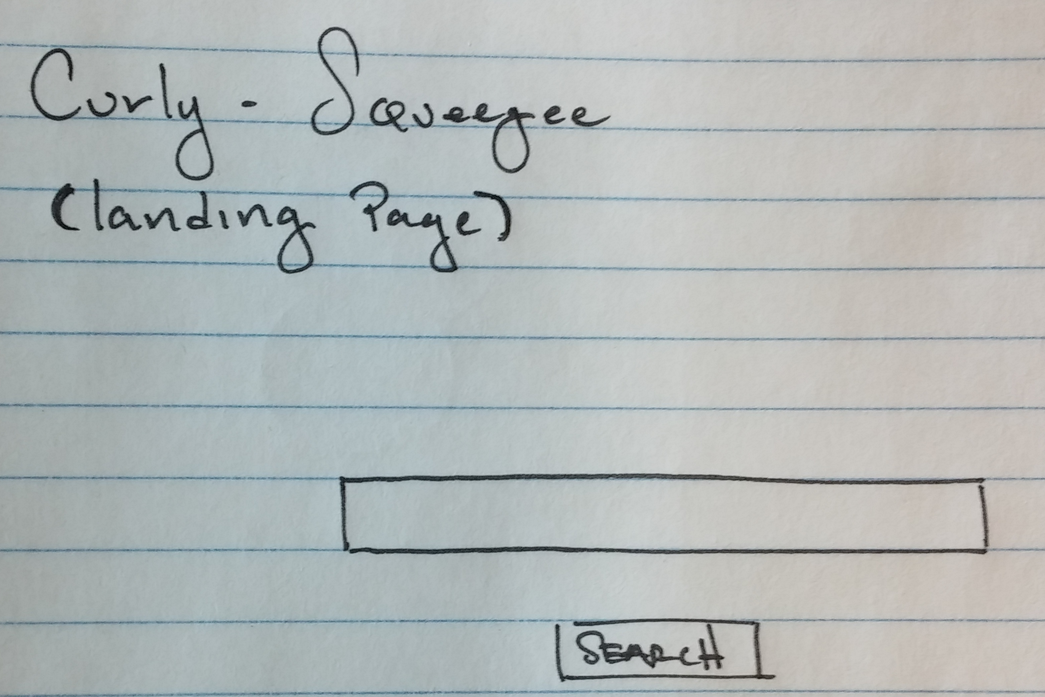
\includegraphics[scale=0.2]{images/landingPage_crop.png}
			  \caption{Original design sketch}
			  \label{fig:sub1}
		\end{subfigure}%
		\begin{subfigure}[t]{.5\textwidth}
			  \centering
			  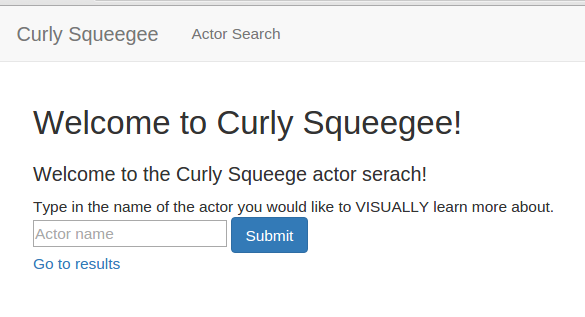
\includegraphics[scale=0.4]{images/landingPage.png}
			  \caption{First implementation}
			  \label{fig:sub2}
		\end{subfigure}%
		\caption{Landing page development}
		\label{fig:landingPage}
	\end{figure}


 


We added some explanatory text to inform users of what they are presented with, and include a navigation bar for ease of moving around the pages. In this first iteration, the user must input the actor they want to search for.  In the redesign (figure \ref{blackLandingPage}) we added an option to select from a list of popular actors.

One serendipitous benefit of using our API calls is that this approach is fairly robust against alternate names and typographical errors.  Searching for actors based on their stage names, nick-names, (or thier misspellings) will return the most-similar actor. Often times the desired result.  

One drawback is that there is currently no disambiguation to select between multiple actors with the same name.  The only choice is to search for a more exact version of the actor's name in the database.

\subsubsection{Site Redesign}


\begin{figure}
\centering
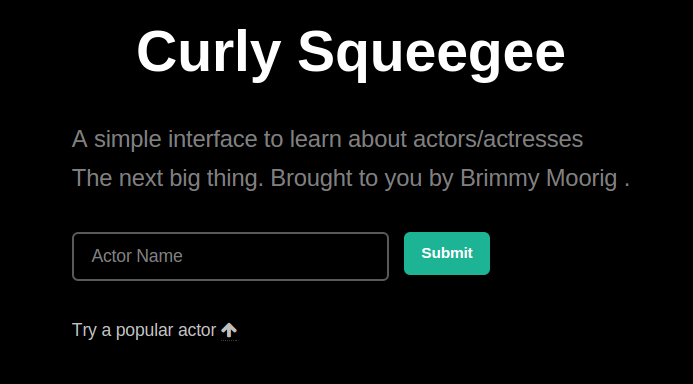
\includegraphics[scale=0.3]{images/landingBoxFinal.png}
\caption{Final version of landing page.}\label{blackLandingPage}
\end{figure}


Once the views were working and the settings more or less finalized, we decided to work on changing the look of the site.  We wanted to keep the same simplistic look, but benefit from some additional polishing from some pre-packaged CSS and JS styling elements. 

Not every page was affected, but we did alter the landing page (Figure \ref{blackLandingPage}) , and modify the scrolling behavior of the results page.  These changes were purely cosmetic and were employed to give the site a more cohesive and smooth look.




We chose a design template from \href{http://html5up.net/}{HTML5 Up} for its stripped-down appearance, and then JS package (\href{http://alvarotrigo.com/fullPage/}{fullPage.js}) for jump-to-view functionality.  Since all of our content lives on one page, we wanted a clean way to transition between views.

\subsection{Loading Page}

Once the user has made their selection, the node.js framework takes that search query and polls the MyAPIFilms' and OMDB's databases to collect the necessary actor information.  Fulilling these requests can take some time, so we display a loading gif to indicate that the process is ongoing.

			\begin{figure}[h!]
				\centering
				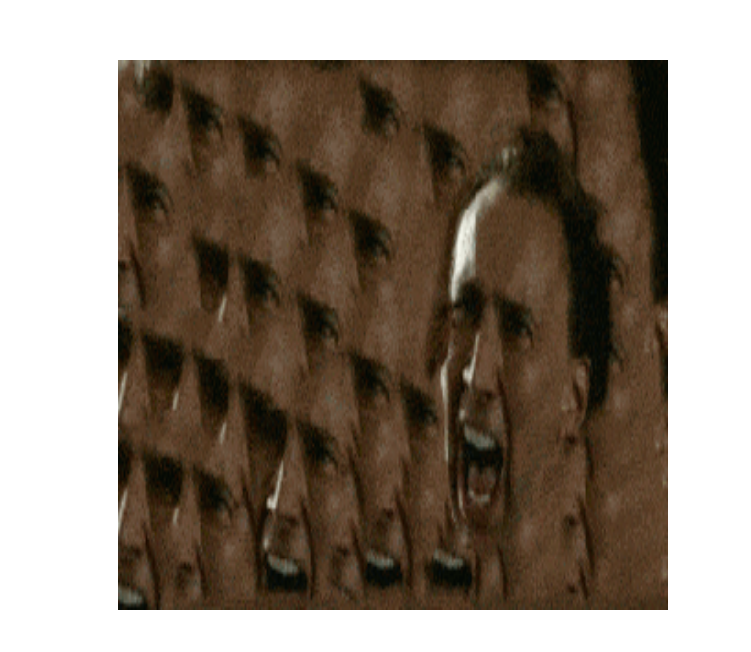
\includegraphics[scale=0.3]{images/loadingPage.png}
				\caption{After the user submits a search query, the application waits for the API calls to complete and fetch the actor's filmography. An animated gif can help pass the time.}
			\end{figure}

The wait times for each search request depend on the extent of the actor's film catalog as well as the user's internet connection.  In our tests, we have experienced wait times as small as a few seconds to upwards of 5 minutes. Typical queiries return within 1-2 minutes.


\subsection{Results Page}

Once the API calls are complete and the data is saved in our database, we load a ``results page'',   showcasing our multiple views and actor information. 

The style of the page is intentionally minimalistic, including a top navigation bar, a small inset photo of the selected actor in the top right, and a Navigation hotlink scroll box on the middle right.

Anatomy of Figure \ref{fig:resultsPage}:


\begin{figure}
	\centering
	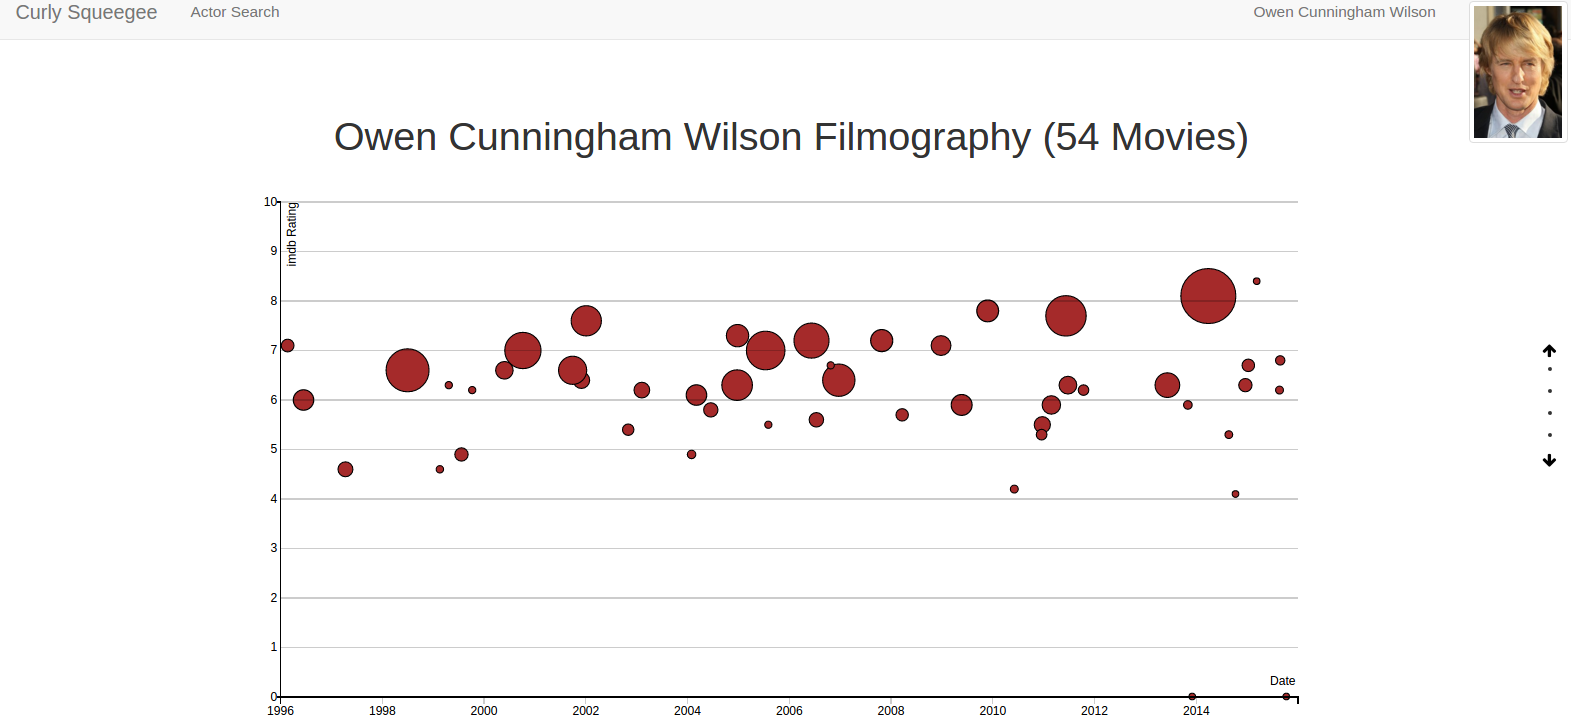
\includegraphics[width = \textwidth]{images/resultsPage.png}
	\caption{Results page layout}\label{fig:resultsPage}
\end{figure}


\begin{itemize}
	\item \textbf{Navigation Bar:}  The top of the page displays links back to the search page, the actor name, and their photo.
	\item \textbf{Main Views:} Each visualization is centered and displayed in its own screen space/ The user can scroll down to view each one, or use the view selector on the right side of the screen. 
	\item \textbf{View Selector:} On the right hand side of the screen, the user can click the stacked dots to jump to any of visualizations.  They may also scroll, and when in the vicinity of the visualization, the browser will auto-center the visualization after a short dwell time.
\end{itemize}

\newpage 

\section{Visualizations}

In this section we go deeper into the visualization choices and design details for each of our chosen views.



\subsection{Actor Fact Box -- Depricated}

\textbf{Note:}  This section was removed from the final release. We decided it did not contribute to the overall presentation and was at odds with the interface style we were hoping to create.  The text remains for  historical analysis.


\textit{ (Depreicated)	This data serves as an orientation tool,indicating to the user whether the correct actor was returned.  This is particularly important in cases when searching for actors with common names.  Using the OMDB API data, we are able to display a photograph of the actor, their full name, date of birth, and other derived data from the API call.  We currently display their total number of films.  other useful information would be when they started acting \textbackslash first credited role, years active, and highest or worst rated movie.}
	
		\begin{figure}[h!]
			\centering
			\begin{subfigure}[t]{.5\textwidth}
				  \centering
				  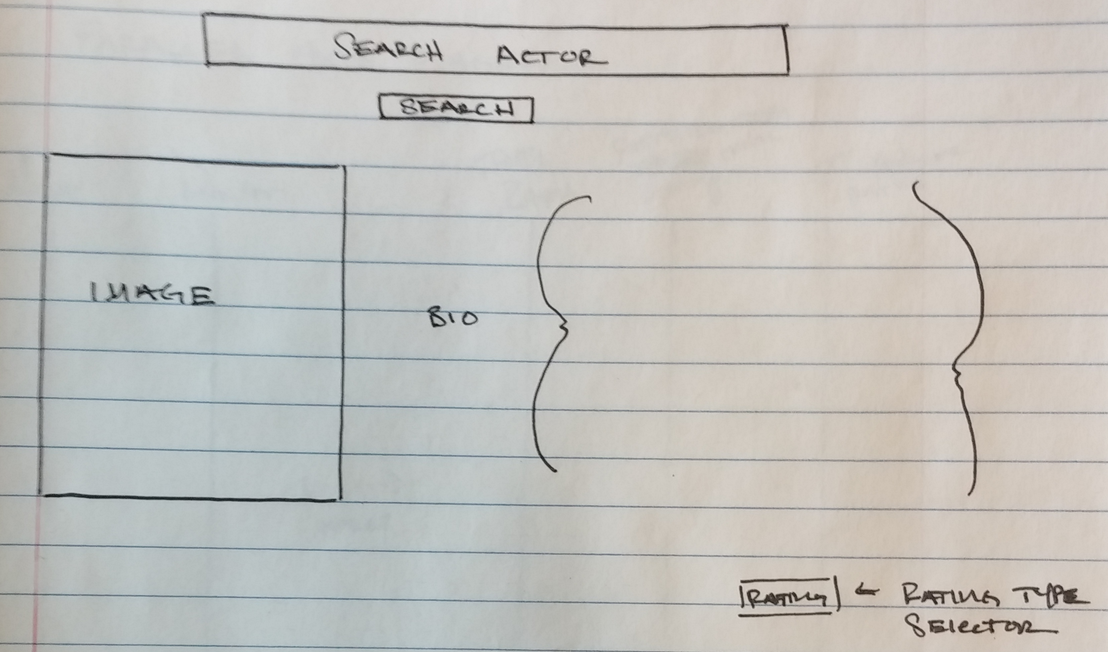
\includegraphics[width=\linewidth]{images/actorFactBox_crop.png}
				  \caption{Original design sketch}
				  \label{fig:sub1}
			\end{subfigure}%
			\begin{subfigure}[t]{.5\textwidth}
				  \centering
				  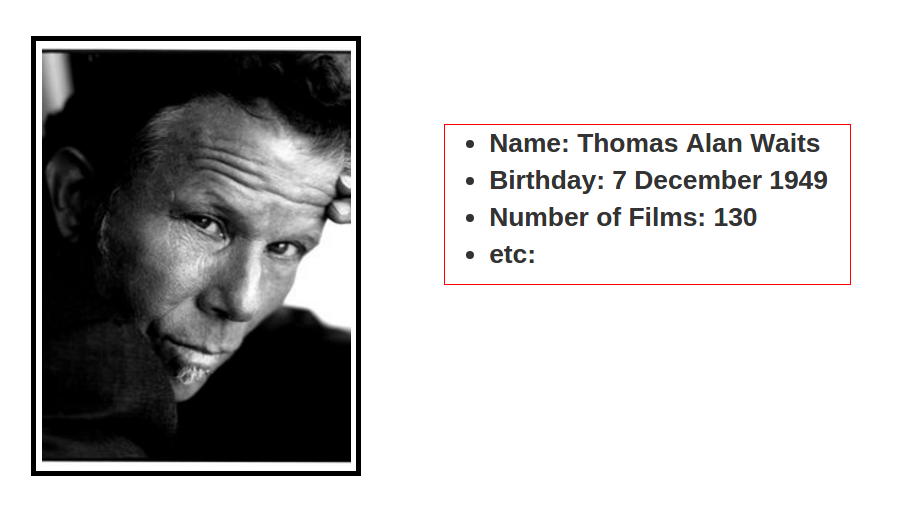
\includegraphics[width=.8\linewidth]{images/actorBox.png}
				  \caption{Original implementation}
				  \label{fig:sub2}
			\end{subfigure}%
			\caption{Actor `Fact Box' development}
			\label{fig:actorFactBox}
		\end{figure}

\newpage

\subsection{Filmography Timeline}


The most natural way to visualize an actor's career is over a timeline.  We considered using circles on a timeline as a suitable encoding for showing film distribution Early in our design phase.  This decision was inspired by the \href{http://mariandoerk.de/edgemaps/demo/#phils;time;;;}{philosophers, poets, and musicians}  visualization shown in class. 

In our original design, we wanted to chroniologically visualize the distribution (and density) of an artist's career and encode information such as film ratings or movie earnings as the circle radius or fill color.   We refined this decision after our brainstorming session (Section \ref{sec:Projcet Feedback}), where concerns were raised that actors with frequent and\textbackslash or successful work would create a cluttered timeline visual.  We also recalled the ineffectiveness of using areas to encode quantitative values for comparison.  When it came time to code our visualization, we decided to switch to a barchart visual.  This way we could cleanly show movie release dates along an $x$ axis and use clearer comparison of quantitative data by mapping it to bar height.

	\begin{figure}[h!]
			\centering
			\begin{subfigure}[t]{.5\textwidth}
			  \centering
			  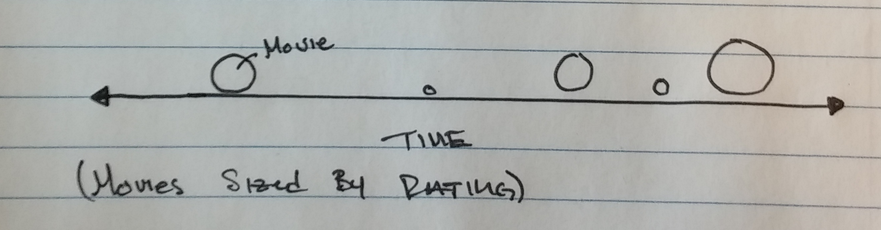
\includegraphics[width=\linewidth]{images/timeline_orig.png}
			  \caption{Original design sketch}
			  \label{fig:timelineA}
			\end{subfigure}%
			\begin{subfigure}[t]{.5\textwidth}
			  \centering
			  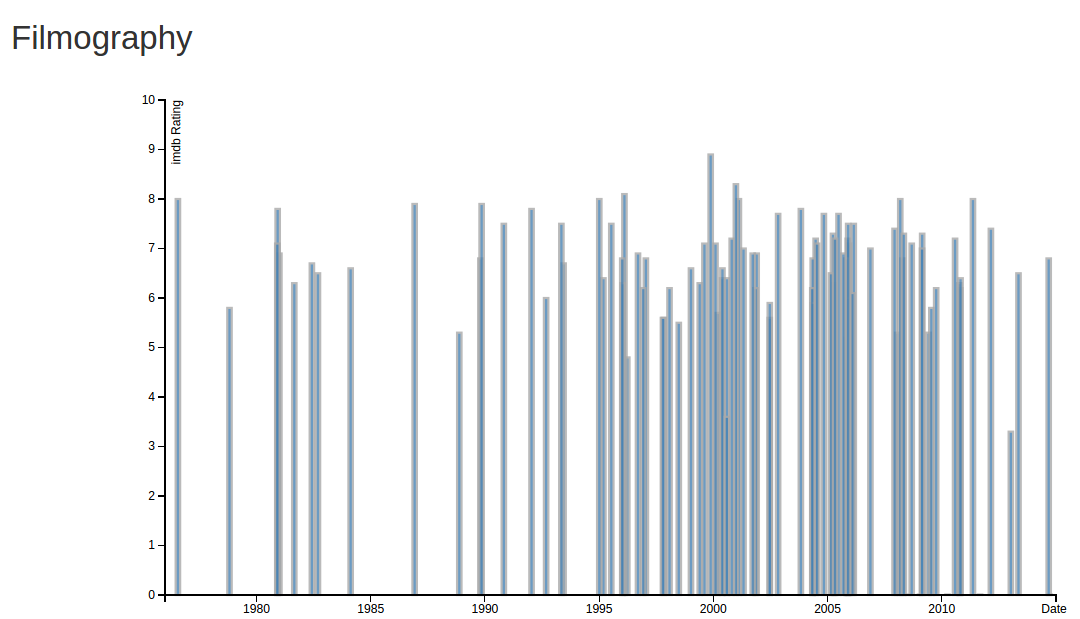
\includegraphics[width=.7\linewidth]{images/timeline_crop_waits.png}
			  \caption{First Implementation}
			  \label{fig:timelineB}
			\end{subfigure}%
			\caption{Timeline development}
			\label{fig:timeline}
		\end{figure}
		
		
Despite this revision, we encountered several issues relating to bar sizing, spacing, and overlap.  When designing this visualization, we did not initially consider cases of long acting careers, high film output, or areas of dense activity (Figure \ref{fig:timelineB}). In each of these regimes, bar sizing and spacing becomes an issue for readability and visual appeal.  Particularly frustrating, were positions where an actor would have multiple films released within a small time frame.  We tried distinguishing these views by using thinner rectangles, adding stroke width to the bars, or introducing opacity.  In the end, we were not happy with any of these solutions and sought a better visualization method.

\begin{figure}
	\centering
	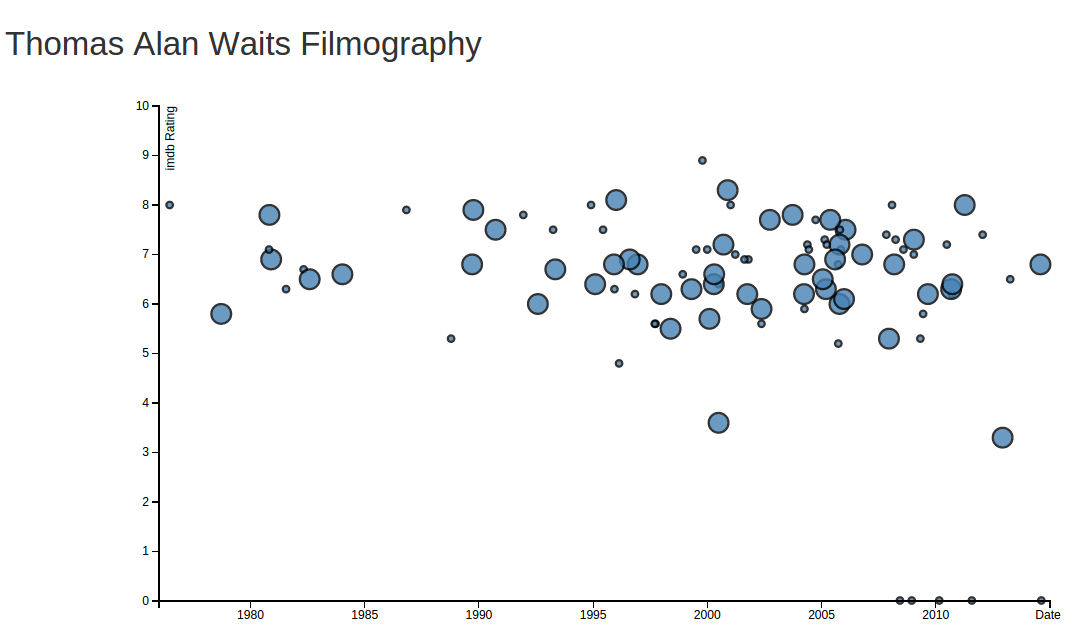
\includegraphics[width=.7\linewidth]{images/timelineC_crop_waits.png}
				  \caption{XY Plot of Tom Waits filmography.  circles are sized by number of  IMDB votes.}
\end{figure}\label{fig:xy}


After realizing we were most interested in showing two values -- release date and rating, we saw this could be arranged as an ordered pair, and thus most effectively plotted on a cartesian grid.  Figure \ref{fig:xy} is a marked improvement over the earlier efforts to illustrate an actor's filmography.  In addition to spatial placement, we encoded the film popularity by its dot size.  Here, popularity is determined by the number of votes it received on its IMDB page.

We feel this view is especially effective as XY plots naturally lend themselves to ordered rankings in each dimension.  This is quickly used to identify information such as : high and low ranked films, popular films, and any trend in the actor's career over time.  For example, figure \ref{fig:deniro} verifies the steady decline of  Robert DeNiro's film quality throughout the 90's.

\begin{figure}
	\centering
	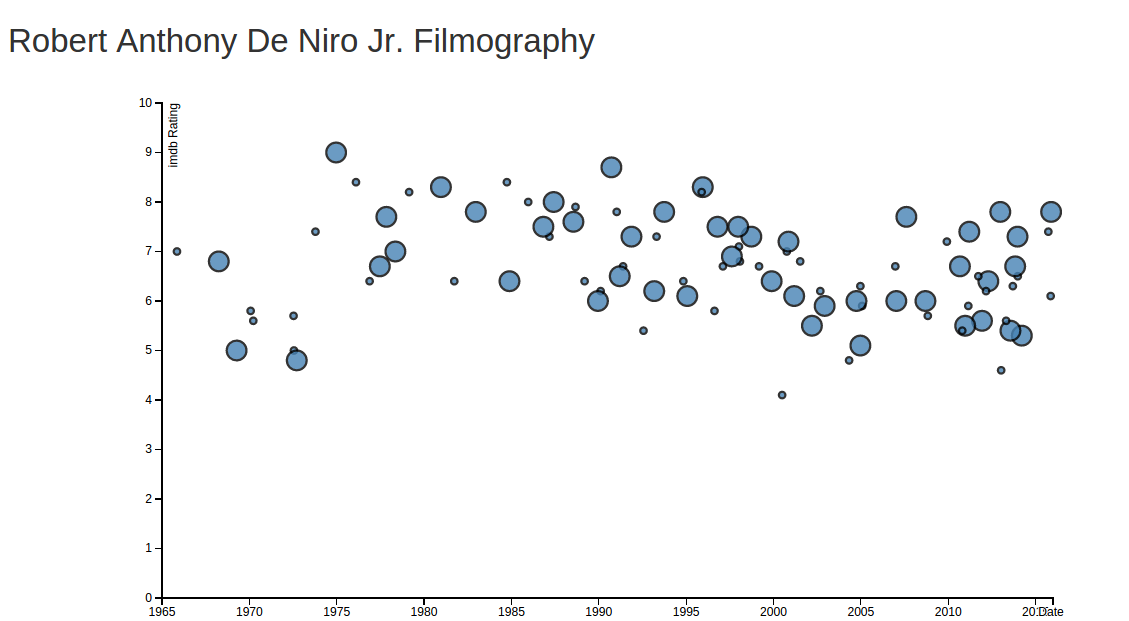
\includegraphics[width=.7\linewidth]{images/Deniro_timeline.png}
				  \caption{Slump in the 90's.}\label{fig:deniro}
\end{figure}

\newpage 

\subsection{Parallel Axis Coordinate Visualization}
	
From the start, the parallel axis coordinate view was what we were most interested in implementing for this dataset. With this view, we can brush over multiple axes to highlight movies fitting arbitrary critea the user can impose.  The films which satisfy these filters are highlighted in blue in the parallel axis chart and also in a contrasting color above in the Filmography timeline.

The code for this visualization was borrowed from the Mike Bostock Block, and we modified it to include the following:

\begin{itemize}
	\item Highlight-on-hover  for each line
	\item Movie title tool tip on hover for each line.
	\item Increase movie title font size on mouse-over for films  in the `Title' axis.
	\item Each axes is scrubable and will highlight any films in the given selection, and those in the filmography.
\end{itemize}

	\begin{figure}[h!]
		\centering
		\begin{subfigure}[t]{.5\textwidth}
			  \centering
			  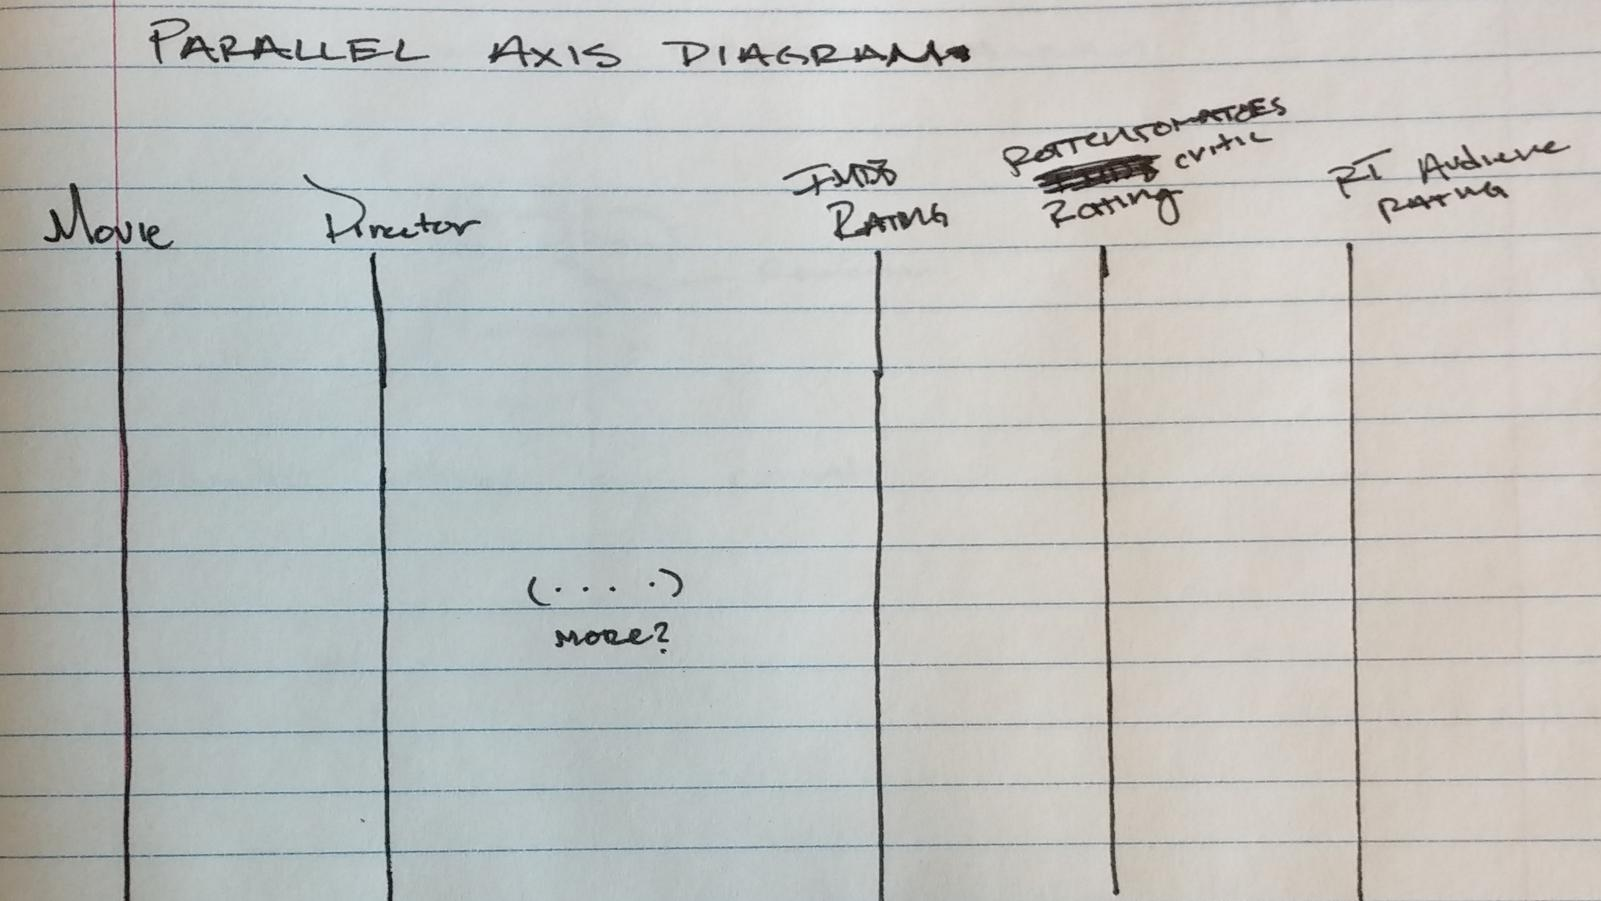
\includegraphics[width=\linewidth]{images/parallel_crop.jpg}
			  \caption{Original design sketch}
			  \label{fig:sub1}
		\end{subfigure}%
		\begin{subfigure}[t]{.6\textwidth}
			  \centering
			  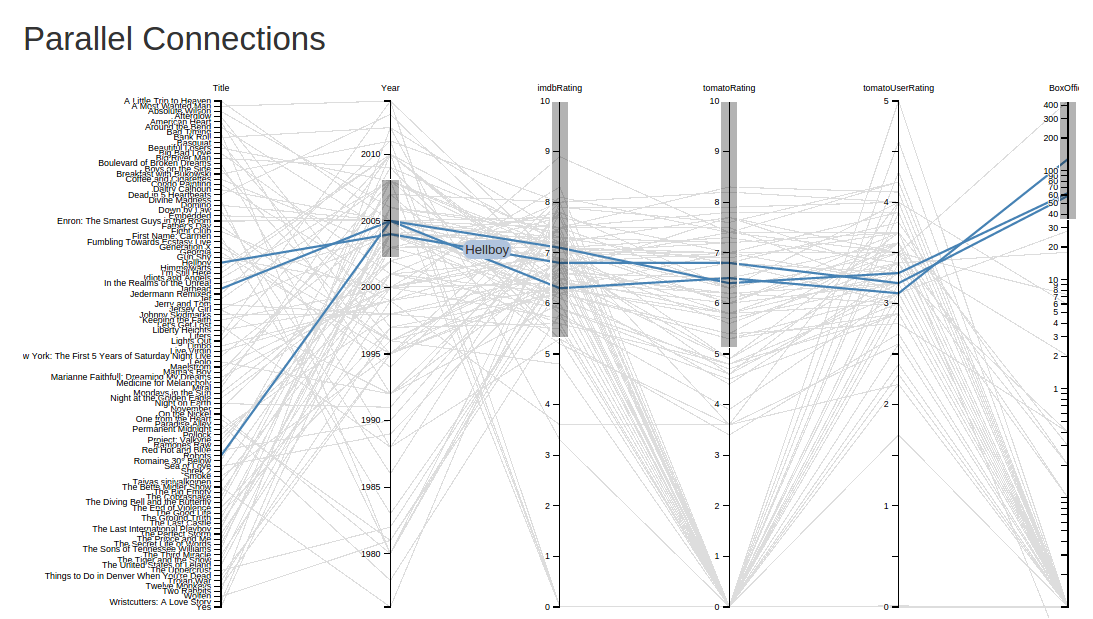
\includegraphics[scale=.2]{images/parallelAxisCoordVis.png}
			  \caption{Current implementation}
			  \label{fig:sub2}
		\end{subfigure}%
		\caption{Parallel Axis Coordinate visualization development}
		\label{fig:parallelAxisCoordVis}
	\end{figure}


\newpage 

\subsection{Treemap Visualization of co-workers}

The treemap visualization was a last-minute addition to our project, inspired by the ``Visualizing Maps and Trees'' lecture.

In this view we catalog the other costars the queried actor stars alongside and sizes each box according to the number of shared films.
	\begin{figure}[h!]
		\centering
		\begin{subfigure}[t]{.5\textwidth}
		  \centering
		  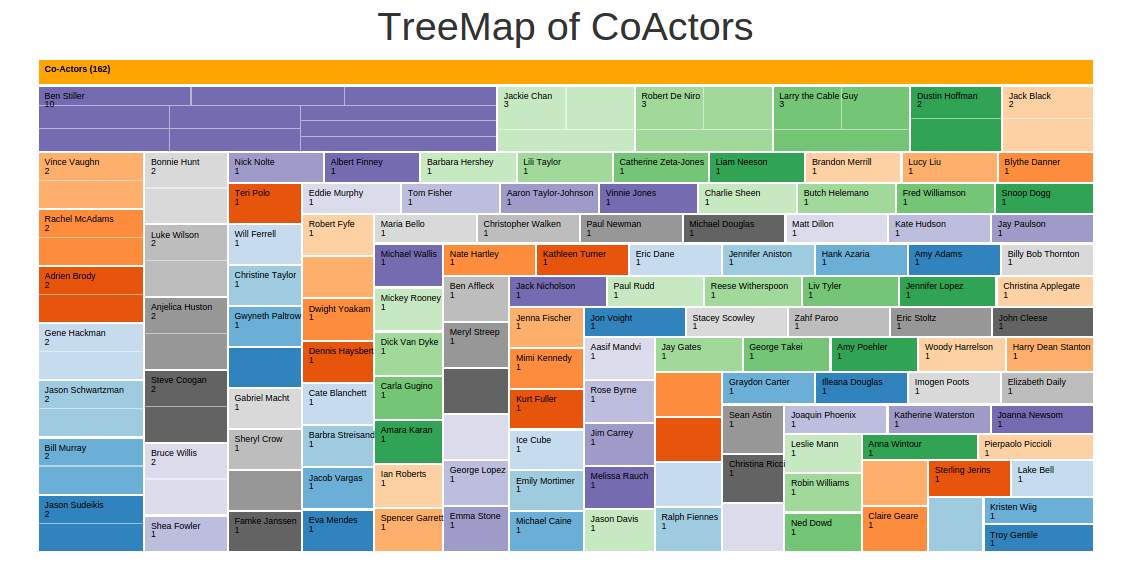
\includegraphics[width=\linewidth]{images/treemapOwenWilson.png}
		  \caption{Collection of co-stars for Owen Wilson.}
		  \label{fig:treemapA}
		\end{subfigure}%
		\begin{subfigure}[t]{.5\textwidth}
		  \centering
		  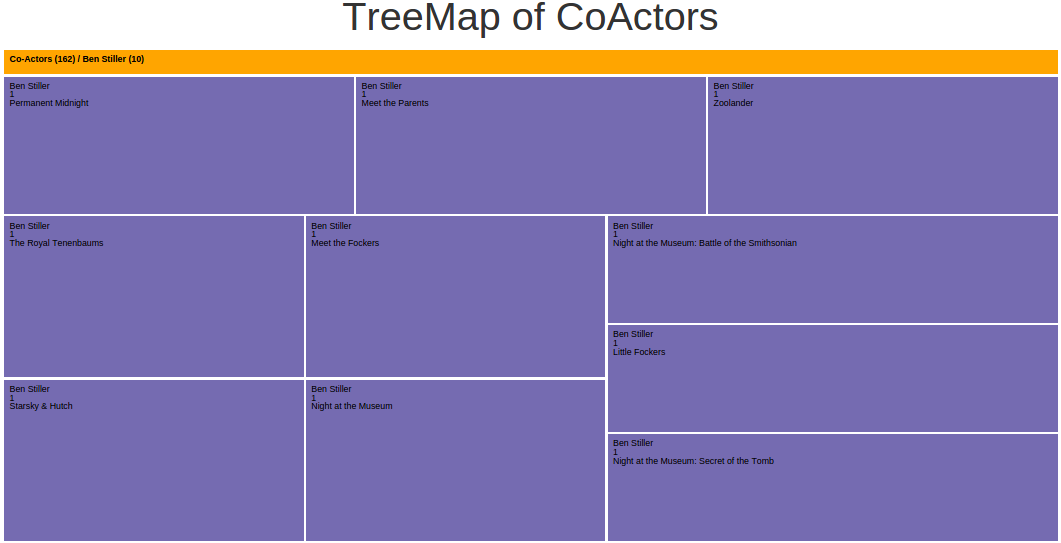
\includegraphics[width=.9\linewidth]{images/treemapZoomWilson.png}
		  \caption{Common films between Owen Wilson and Ben Stiller}
		  \label{fig:treemapB}
		\end{subfigure}%
		\caption{Tree Map visualization for Owen Wilson's career}
		\label{fig:Treemap}
	\end{figure}
		
The tree map supports one zoomable level, to drill down and see a list of the movies the two actors share.
\newpage

\subsection{Genre Visualization}

	\begin{figure}[h!]
		\centering
		\begin{subfigure}[t]{.5\textwidth}
		  \centering
		  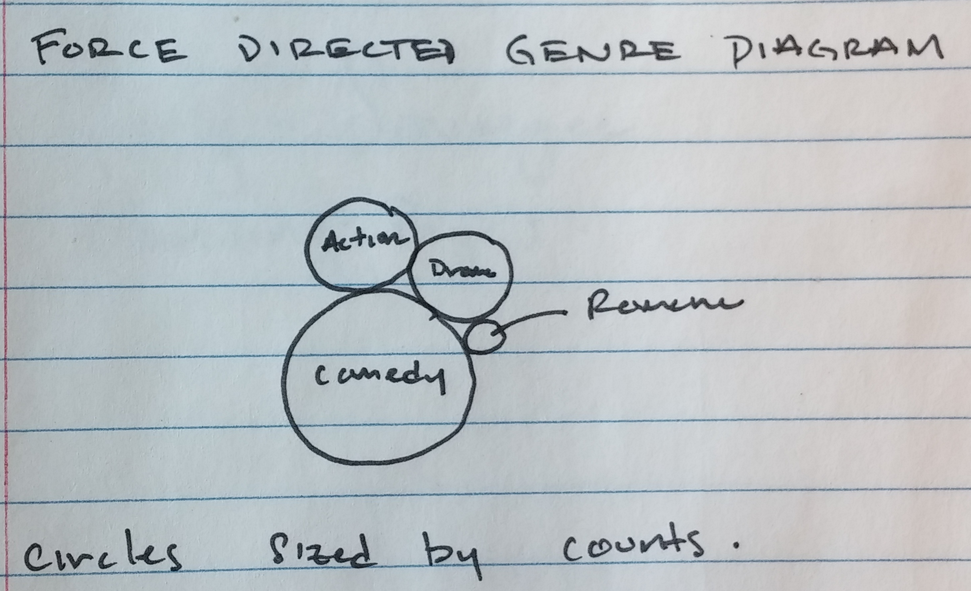
\includegraphics[width=\linewidth]{images/genreVis_crop.png}
		  \caption{Original design sketch}
		  \label{fig:sub1}
		\end{subfigure}%
		\begin{subfigure}[t]{.5\textwidth}
		  \centering
		  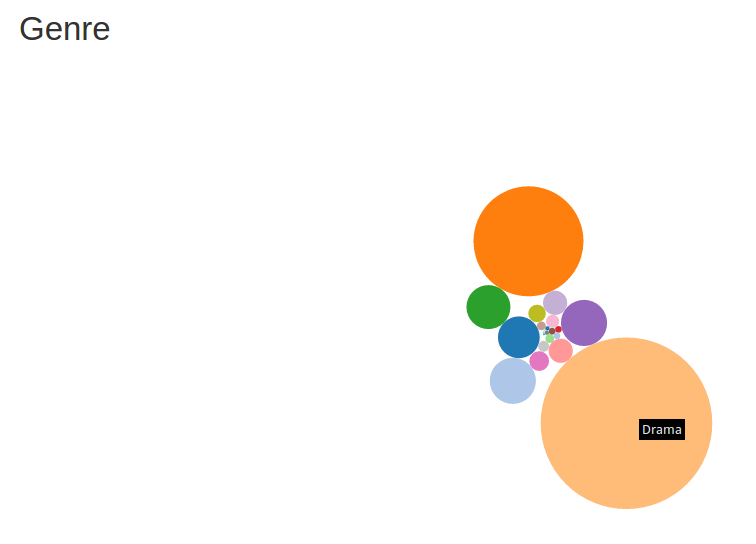
\includegraphics[width=.9\linewidth]{images/genreVis.png}
		  \caption{Current implementation}
		  \label{fig:sub2}
		\end{subfigure}%
		\caption{Genre visualization development}
		\label{fig:genreVis}
	\end{figure}

	
The GenreVis view (figure \ref{fig:genreVis}) was created to visualize an actor's breadth of work or whether they are disproportionately cast one type of genre.  

In this view, each circle represents a unique film genre (Drama, family, comedy, etc.) which is viewable via mouse-hover text.  To create this view, we parsed every film genre lable in the actors filmography and added unique labels to an array.  We counted the number of times each label appeared, and sized the circles accordingly.  Films which had multiple or compound genres ('action thriller' or `romantic comedy' ) would count each descriptor towards the actors genre aggregate.


	\begin{figure}[h!]
		\centering
		\begin{subfigure}[t]{.5\textwidth}
		  \centering
		  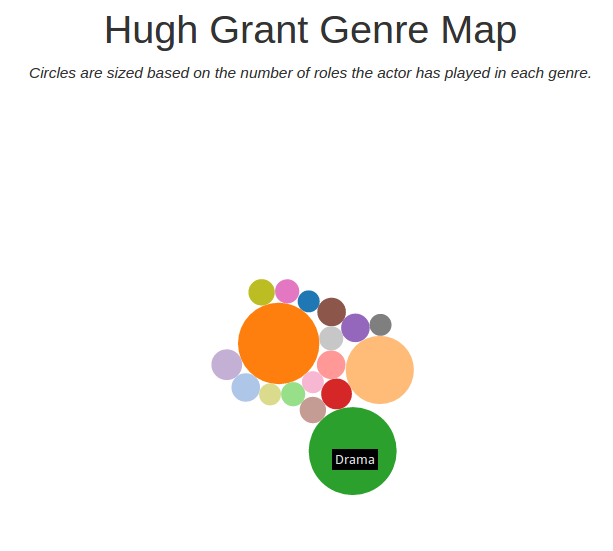
\includegraphics[width=\linewidth]{images/HughGrantGenre.png}
		  \caption{ Hugh Grant.  The Other large orange dot is `Romance'.}
		  \label{fig:HughGrantGenre}
		\end{subfigure}%
		\begin{subfigure}[t]{.5\textwidth}
		  \centering
		  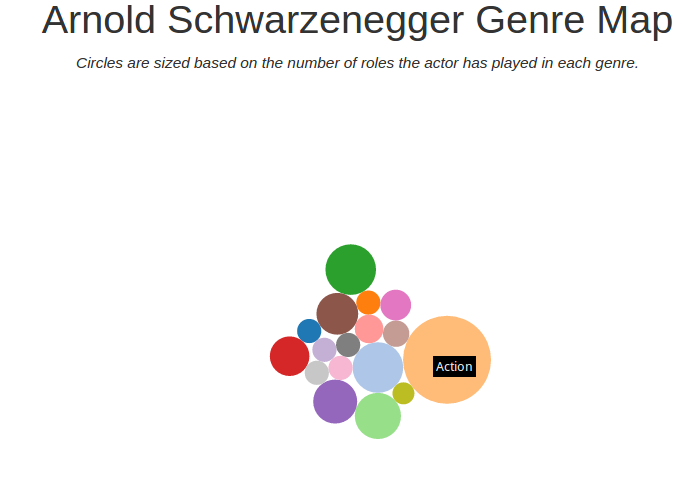
\includegraphics[width=\linewidth]{images/ArnoldGenreVis.png}
		  \caption{Ahnold.  No surprises here.}
		  \label{fig:ArnoldGenre}
		\end{subfigure}%
		\caption{specific Actor Genre visualizations }
		\label{fig:CharacterGenreVis}
	\end{figure}


\newpage



\section{Connected Views}

To make the main views more interactive, we used the broadcast model of event handling from homework 4 to connect our filmography and Parallel Axis views. Selecting films in one of the views will highlight the corresponding entry in the other view.  Brushing in parallel axis view will highlight multiple films in the timeline (figures \ref{fig:filmToParallelHighlight}, 
\ref{fig:parallelToFilmHighlight}).

These connected views are especially useful when applying multiple filters in the parallel axis coordinate view and seeing the highlighted distribution of films in the timeline graphic.

We thought this functionality would help uncover actor trends.  For instance, the bulk of Will Smith's highest grossing movies all occur in 2000-2010 (figure \ref{fig:ptfhb} ).

\begin{figure}[h!]
		\centering
		\begin{subfigure}[t]{.5\textwidth}
		  \centering
		  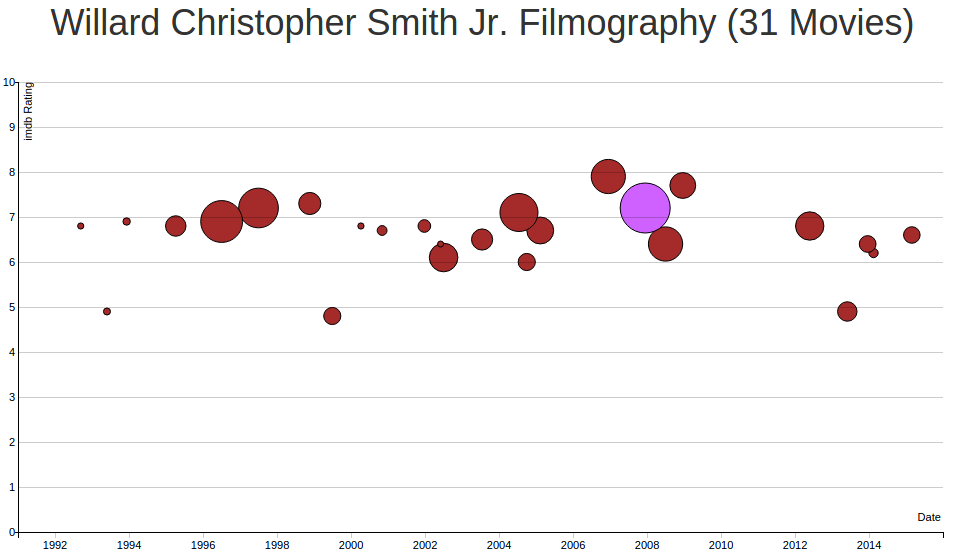
\includegraphics[width=\linewidth]{images/TimelineSelection.png}
		  \caption{User-selected movie from Will Smith's Filmography}
		  \label{fig:ftpha}
		\end{subfigure}%
		\begin{subfigure}[t]{.6\textwidth}
		  \centering
		  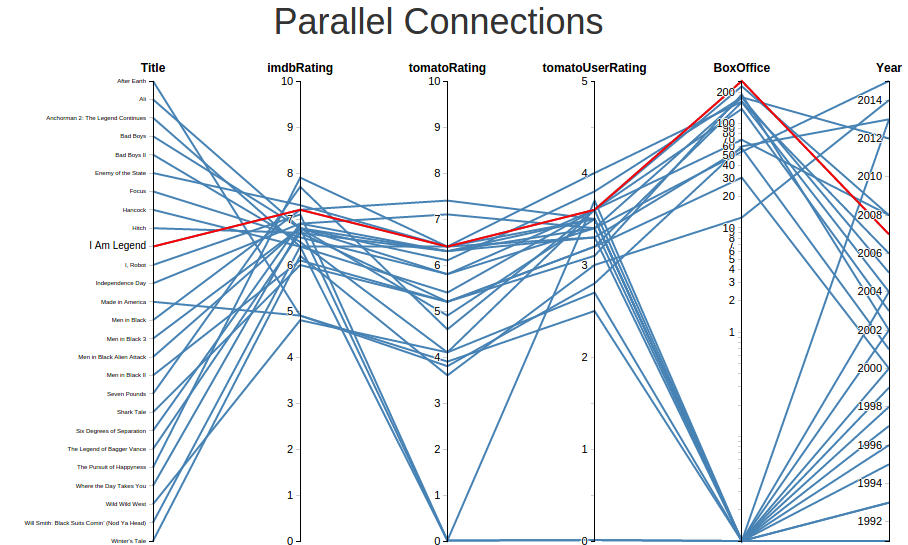
\includegraphics[width=\linewidth]{images/pacHighlight.png}
		  \caption{Also highlighted in the Parallel Connections View}
		  \label{fig:ftphb}
		\end{subfigure}%
		\caption{Event-driven highlighting.  Selections from the Filmography are highlighted in the Parallel Connection view.}
		\label{fig:filmToParallelHighlight}
	\end{figure}


	\begin{figure}[h!]
		\centering
		\begin{subfigure}[t]{.5\textwidth}
		  \centering
		  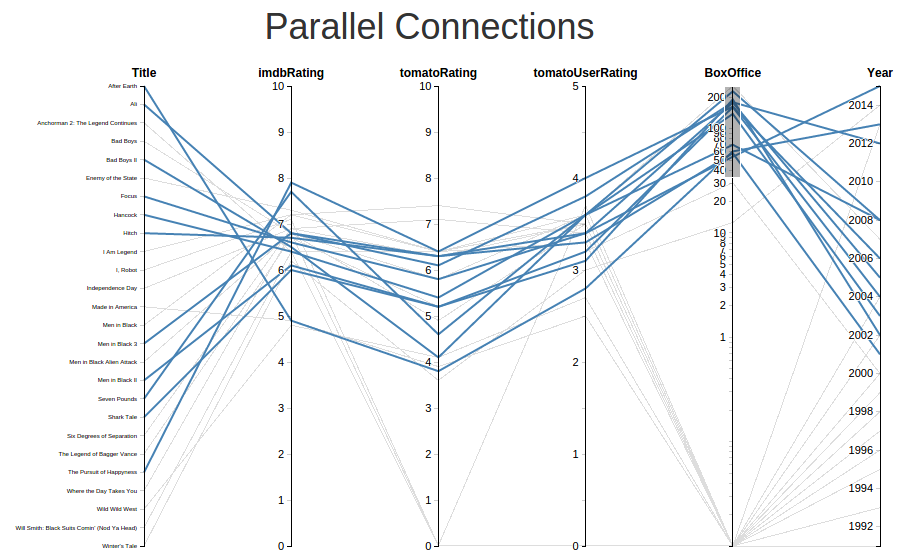
\includegraphics[width=\linewidth]{images/pacScrub.png}
		  \caption{User-brushed selection from Parallel Connections view.}
		  \label{fig:ptfha}
		\end{subfigure}%
		\begin{subfigure}[t]{.6\textwidth}
		  \centering
		  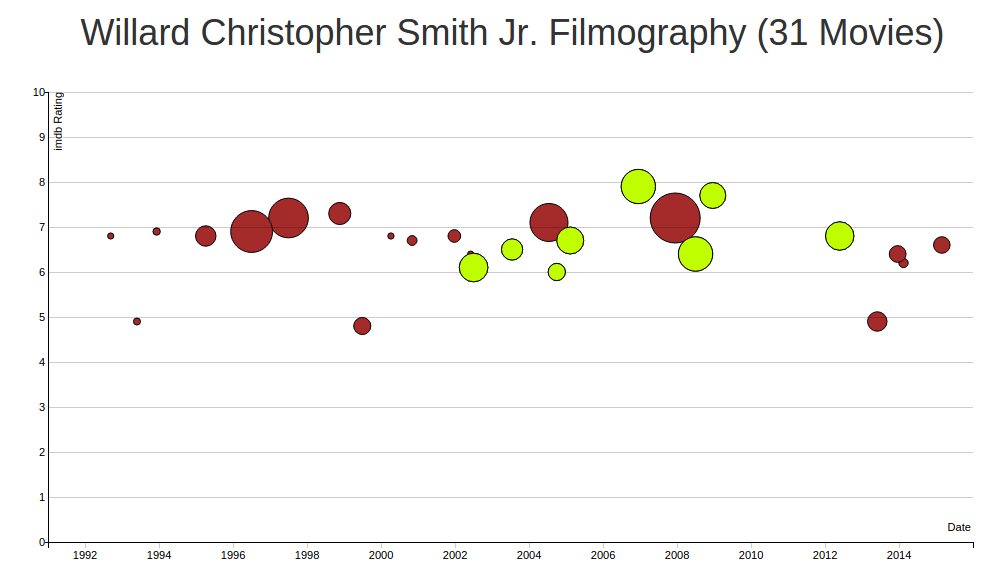
\includegraphics[width=\linewidth]{images/TimelinePacHighlight.png}
		  \caption{Also highlighted in the Parallel Connections View}
		  \label{fig:ptfhb}
		\end{subfigure}%
		\caption{Event-driven highlighting.  Selections from the Filmography are highlighted in the Parallel Connection view.}
		\label{fig:parallelToFilmHighlight}
	\end{figure}
	
	
\newpage

\section{Project Feedback} \label{sec:Projcet Feedback}

We had the opportunity to present a Curly-Squeegee to another project team after we settled on our project design.   We pitched our Idea to Phil Cutler, Ariel Herbert-Voss, and Ian Sohl of the "Legion Profiling Visualization" team. They provided the following feedback:

\begin{itemize}
	\item \textbf{Phil Cutler} (u0764757@utah.edu)
	
	Provided good feedback and constructive criticism. Raised concerns about Parallel axis plot readability in the limit of a long, active acting career as well as a lack of information on new actors. Liked the idea of the filmography visualization, but recommended using bar charts as opposed to circles anchored to a timeline. He thought it was a neat idea, but did not see it's utility. He admitted he does not like watching movies.
	
	
	\item \textbf{Ariel Herbert-Voss} (u0591949@utah.edu)
	
	Overall very positive and excited reaction. she loved the parallel axis plot idea and also agreed with Phil that a bar chart for the filmography timeline would be more effective. She suggested scaling bars either by film rating or number of films in a given period (for a drill-down style barchart), as well as shading a given bar to convey additional information. Ariel is a film buff and saw a great deal of utility in this visualization
	
	\item \textbf{Ian Sohl} (u0445696@utah.edu)
		No additional feedback beyond what Phil and Ariel had to suggest.
\end{itemize}

\newpage

\section{Team Evaluation}

\textit{Brian Kimmig}: Brian was responsible for the managing the preliminary API calls, data collection, and database wrangling. His experience as a web developer was very helpful for making this portion of the project proceed smoothly. Brian also created  the genreVis, treep map, and parallel coordinate view.

\textit{Jimmy Moore}: Jimmy contributed code for the Database storage of API calls, the actor filmography visualization, and with site formatting.  He also was the project scribe and responsible for proposal and final report documentation.

\newpage

\section{Future Work}


We both are excited at the direction this project could take with some more time.  There are several areas which work well enough, but which we could see being more user-friendly or thouroughly fleshed out:


\begin{enumerate}

	\item Timeline view:
		\begin{itemize}
			\item extend search to other roles (Director, etc.) and add a selector to change search query from visualizing filmography to other directorial roles, soundtrack, or other creative capacity.  
			\item Allow support for searching and overlaying multiple actors. color the points and overlay them to compare the activity and success of multiple people.
		\end{itemize}
		
	\item Parallel axis view
		\begin{itemize}
			\item Add different axes to filter against
			\item Collect additional film data (perhaps from a separate source) to fill in Box office earings numbers which appear to be missing from a majority of the API calls.
		\end{itemize}
	
	\item: Treemap view
		\begin{itemize}
			\item General cleanup  and exploring other shapes
			\item Link view to highlight corresponding films in the Filmography Timeline
		\end{itemize}

	\item Genre view
		\begin{itemize}
			\item Create a legend for the various colors
			\item Explore other methods of displaying this information (Bar charts?)
			\item Label the dots directly
			\item Link view to highlight corresponding films in the Filmography Timeline
		\end{itemize}
	\item Additional views
		\begin{itemize}
			\item Create a set view to show which movies any $n$ actors have acted in.  Or show a network visualization of the separation of a number of actors.  Use the individual movies as the graph nodes.  Force directed visualization might be best.
		\end{itemize}
\end{enumerate}

\end{document}